\section{Какие сведения должен сохранять рантайм}
\label{sec:runtime}
\subsection{Наблюдения среды и семантическая память}
Среда исполнения уже получает результаты инструментов. Ей не требуется вызывать модель, чтобы сохранить команду и доступный вывод. Модель, напротив, нужна для выбора гипотезы, объяснения ошибки и планирования работы. Гибридное состояние разделяет эти обязанности: автоматические записи $V$ хранят захваченные наблюдения, семантическое состояние $S$ --- их интерпретацию и незавершённую работу (рис.~\ref{fig:runtime-written}).

% Adapted from the repository's original state-ownership diagram.
\begin{figure}[tbp]
\centering
\resizebox{\linewidth}{!}{%
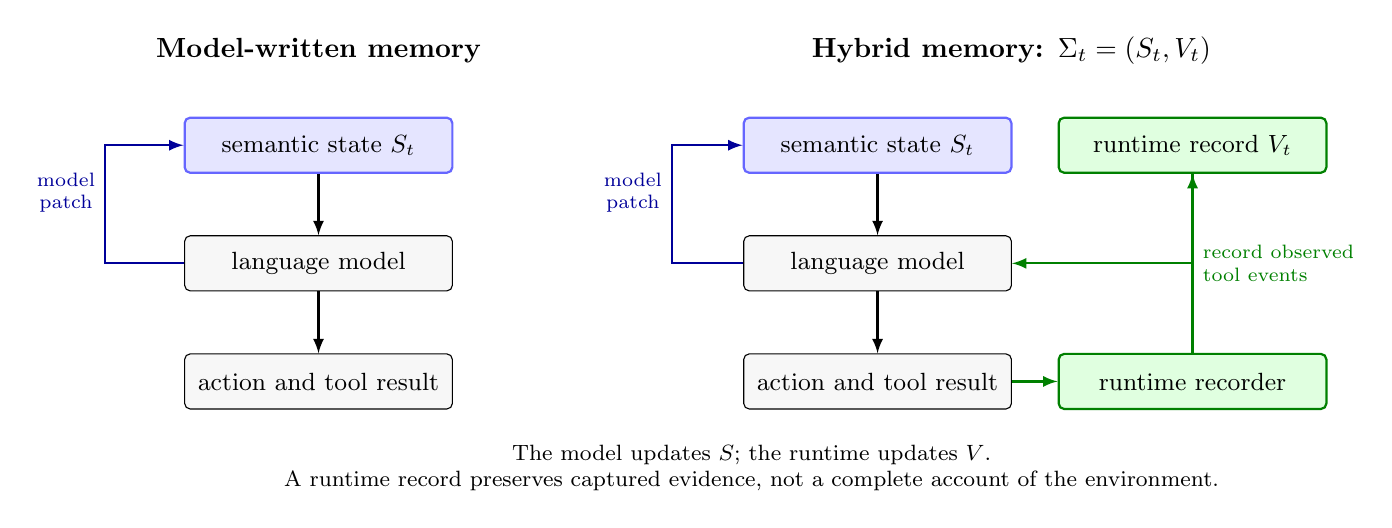
\begin{tikzpicture}[
font=\small,
box/.style={draw,rounded corners=2pt,minimum width=3.4cm,minimum height=.7cm,align=center,inner sep=3pt},
state/.style={box,fill=blue!10,draw=blue!60,thick},
record/.style={box,fill=green!12,draw=green!50!black,thick},
plain/.style={box,fill=black!3},
arr/.style={-latex,thick}]
\node[font=\bfseries] at (0,3.5) {Model-written memory};
\node[state] (s1) at (0,2.3) {semantic state $S_t$};
\node[plain] (m1) at (0,.8) {language model};
\node[plain] (a1) at (0,-.7) {action and tool result};
\draw[arr] (s1)--(m1);
\draw[arr] (m1)--(a1);
\draw[arr,blue!60!black] (m1.west)--++(-1,0)|-(s1.west)
node[pos=.3,left,font=\scriptsize,align=center]{model\\patch};
\begin{scope}[xshift=7.1cm]
\node[font=\bfseries] at (1.7,3.5) {Hybrid memory: $\Sigma_t=(S_t,V_t)$};
\node[state] (s2) at (0,2.3) {semantic state $S_t$};
\node[record] (v2) at (4,2.3) {runtime record $V_t$};
\node[plain] (m2) at (0,.8) {language model};
\node[plain] (a2) at (0,-.7) {action and tool result};
\node[record] (rec) at (4,-.7) {runtime recorder};
\draw[arr] (s2)--(m2);
\draw[arr,green!50!black] (v2.south)|-(m2.east);
\draw[arr] (m2)--(a2);
\draw[arr,blue!60!black] (m2.west)--++(-.9,0)|-(s2.west)
node[pos=.3,left,font=\scriptsize,align=center]{model\\patch};
\draw[arr,green!50!black] (a2)--(rec);
\draw[arr,green!50!black] (rec)--(v2)
node[midway,right,font=\scriptsize,align=left]{record observed\\tool events};
\end{scope}
\node[font=\footnotesize,align=center] at (5.5,-1.8)
{The model updates $S$; the runtime updates $V$.\\A runtime record preserves captured evidence, not a complete account of the environment.};
\end{tikzpicture}}
\caption{State ownership. Hybrid memory retains model-written semantic content and adds runtime-derived records. Recording an event does not establish that an extracted interpretation is correct or that all relevant events were captured.}
\label{fig:runtime-written}
\end{figure}


Такое разделение предлагает конкретный способ уменьшить издержки ведения памяти. Сведения, сохранённые средой исполнения, не требуется заново генерировать в семантическом блоке; модель также не может стереть их своим обновлением $S$. Но объём и содержание $V$ остаются проектными решениями. Один список файлов не заменяет результатов команд, а накопление всех доступных записей увеличивает вход. Поэтому проверять нужно не только наличие автоматической памяти, но и её состав.

\subsection{Состав автоматических записей: поисковое сравнение}
Сравниваются накопительные наборы сведений при неизменных настройках схемы, отдельном инструменте обновления и отсутствии недавней истории. Минимальная конфигурация сохраняет ссылки на затронутые файлы. Следующая добавляет записи изменений и команд с их выводом. Более полная конфигурация включает также диагностики, сведения о среде и результаты тестов; последняя добавляет записи неудачных попыток. Промежуточные компоненты не исследованы по отдельности, поэтому каждый измеренный переход характеризует весь добавленный набор.

\begin{table}[htbp]
\centering\small
\caption{Exploratory comparison of cumulative runtime records, without recent history. Output and cost are medians over all retained executions. Solved/\$ uses aggregate cost, including failures. Exploratory first-repeat subset; the control and richer configurations also contribute to the final comparison.}
\label{tab:composition}
\input{../paper/tables/new-composition}
\end{table}

Переход от ссылок на файлы к записям изменений и команд сопровождается ростом успешности с \ExploreFilesRate\% до \ExploreCommandsRate\% и снижением медианного выхода с \ExploreFilesOutputMedian{} до \ExploreCommandsOutputMedian{} тысяч токенов. Это наиболее выраженное изменение в данном сравнении. Дополнение диагностик, среды и тестов даёт \ExploreRichRate\%, а неудачных попыток --- \ExploreFailuresRate\%; полная история достигает \ExploreControlRate\%.

% Descriptive component comparison; not an independent replication.
\begin{figure}[tbp]
\centering
\begin{tikzpicture}
\begin{axis}[
width=.47\linewidth,height=5.4cm,
title={Task success},title style={font=\small},
ylabel={Solved rate (\%)},ymin=20,ymax=60,
xmin=-.4,xmax=3.4,xtick={0,1,2,3},
xticklabels={{File\\references},{+ action\\records},{+ context\\records},{+ failure\\records}},
xticklabel style={font=\scriptsize,align=center},yticklabel style={font=\scriptsize},
label style={font=\small},grid=major,grid style={black!12},
legend style={font=\scriptsize,at={(.03,.97)},anchor=north west,draw=none,fill=white}]
\addplot[only marks,mark=*,mark size=2.5pt,blue!65!black]
table[col sep=comma,x=order,y=solved_pct]{../paper/generated/new-composition.csv};
\addlegendentry{Hybrid memory}
\addplot[dashed,black!65,domain=-.4:3.4] {\ExploreControlRate};
\addlegendentry{Full history}
\end{axis}
\begin{axis}[
at={(.52\linewidth,0)},anchor=south west,
width=.47\linewidth,height=5.4cm,
title={Cost efficiency},title style={font=\small},
ylabel={Solved/\$},ymin=10,ymax=26,
xmin=-.4,xmax=3.4,xtick={0,1,2,3},
xticklabels={{File\\references},{+ action\\records},{+ context\\records},{+ failure\\records}},
xticklabel style={font=\scriptsize,align=center},yticklabel style={font=\scriptsize},
label style={font=\small},grid=major,grid style={black!12}]
\addplot[only marks,mark=square*,mark size=2.5pt,green!45!black]
table[col sep=comma,x=order,y=solved_per_dollar]{../paper/generated/new-composition.csv};
\addplot[dashed,black!65,domain=-.4:3.4] {\ExploreControlSolvedPerDollar};
\end{axis}
\end{tikzpicture}
\caption{Exploratory comparison of cumulative runtime-owned information. Each
position adds records to the preceding configuration: action records cover
file changes and commands; context records cover diagnostics, environment,
and tests. Efficiency
includes the cost of unsuccessful episodes. Dashed lines show the same
full-history reference. These descriptive observations share their richer
configurations and reference with the first repeat of the final comparison;
they do not isolate individual components or establish a monotonic benefit.}
\label{fig:composition}
\end{figure}


Экономическая картина согласуется с преимуществом содержательных записей перед бедной памятью. Число наблюдаемых успехов на доллар возрастает с \ExploreFilesSolvedPerDollar{} до \ExploreCommandsSolvedPerDollar{} уже после добавления изменений и команд. При этом дальнейшее обогащение не улучшает одновременно все показатели. Медианная стоимость не убывает монотонно, и ни один вариант не достигает успешности полной истории.

Это поисковый результат, а не подтверждённая последовательность независимых компонентных эффектов. Конфигурации с меньшей успешностью не продолжили измерять; сравнение поэтому сохраняет статус предварительного отбора. Оно мотивирует исследование содержимого памяти, но не устанавливает, какой отдельный компонент вызвал прирост или сколько выходных токенов удалось сэкономить именно на записи фактов.

\subsection{Проверка цены и дополнительной памяти о неудачах}
Условный выигрыш по стоимости чувствителен к выбору задач. Для богатой памяти без записей неудач медианное отношение к контролю на собственном подмножестве общих успехов равно \ExploreRichVariableCostRatio{}. Если оставить одинаковое подмножество задач, успешных при всех конфигурациях, отношение становится \ExploreRichFixedCostRatio{}; для максимального набора записей --- \ExploreFailuresFixedCostRatio{}. Снижение издержек относительно памяти со ссылками на файлы сохраняется, но экономия относительно полной истории неустойчива к этому выбору. Полное сопоставление приведено в приложении~\ref{app:composition}.

Повторное сравнение полных гибридных вариантов проверяет более узкое изменение: добавление записей неудачных попыток (табл.~\ref{tab:runtime}). Успешность составляет \HybridNoFailureRate\% без таких записей и \HybridRate\% с ними; прямое сравнение даёт $p=\HybridNoFailureVsHybridP$. Заметного дополнительного выигрыша здесь не установлено.

\begin{table}[htbp]
\centering\small
\caption{Repeated comparison of hybrid state with and without failure records. Output, cache reads and cost are per-execution medians. Token counts are in thousands; table $p$-values compare each policy with full history.}
\label{tab:runtime}
\input{../paper/tables/new-runtime}
\end{table}

Состав памяти оказался содержательным направлением поиска: бедные ссылки и записи результатов действий дают разные результаты. Но автоматическое сохранение фактов не устранило отставание от полной истории. Следующий вопрос касается информации, которая остаётся в самих взаимодействиях и может не попасть ни в семантический блок, ни в набор автоматических полей.
